\section{Nuclei mass measurements with regard to nuclear force theory}
This section looks extensively into the Nucleon pairing energy, nuclear mass measurements and magic numbers.
Analysis of nucleon binding energies is achieved by investigating the magic numbers of nucleons.
The magic number represents stable atoms that are less likely to be radioactive. 
Before discovering the standard 2, 8, 30, 28, 50, 82, 126 magic numbers, higher values of 184, 258, 350, and 462 are thought to exist. 
The existence of these number are predicted and are calculated based on the Binomial coefficient.
\subsection{Nucleon pairing energy}
The energy to add a single nucleon (neutron in this case) to the nucleus is given by \cref{eq:NMMwrtNFTSn} also shown in \cref{fig:MSaNFTzigzag}.
For two nucleon energy the equation becomes:

\begin{equation}\label{eq:NMMwrtNFTSn}
    S_{2n} = M_{a}(N-2,Z) + 2M_{n} - M_{a}(N,Z)
\end{equation}

The $S_{2n}$ is the binding energy of two nuclei, $M_{a}$ is the atomic mass N is the nucleon number, and $M_n$ is nucleon mass, and Z is the proton number.  
Looking at the Nucleon pairing energy makes more sense because it reduces the graph's noise. 
From \cref{fig:MSaNFTzigzag} the graph shows a zigzag pattern which is difficult to analyse. 
The data is much smoother with a Nucleon pairing energy graph, making it easy to analyse.  
Besides the standard investigations, we can also investigate the neutron pairing energy of finite nuclei.
We can study a range of odd and even pairs of N/Z numbers; to investigate the strong nuclear force \cite{fred_neutron_2019}.
So far, the idea is that the (N)even-(Z)even nucleus (although energy depends on factors such as the kind of particles and state it is occupied) we known for a fact that odd(N)- odd(A) nucleus is 1/2 to 2/3 times smaller, this is when they are given in the same shell. The mass numbers A are very close to one another.
This strange character is due to the nucleon-nucleon potential resulting from the strong force. \cite{jensen_elementary_1955}

\begin{figure}[H]
    \centering
    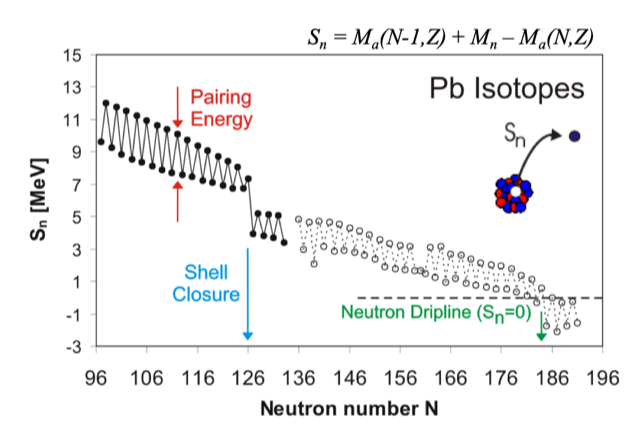
\includegraphics[width=.5\textwidth]{images/NMMwrtNFT_zigzag.png}
    \caption{Neutron binding energy for lead isotopes. In blue a shell closure is highlighted at 126N. The sharp oscillations in energy highlight neutron pairing energies \cite{noauthor_nuclear_nodate}.}\label{fig:MSaNFTzigzag}
\end{figure}

The binding energy of magic nuclei refers to when N or Z are a magic number; for the stable atoms, these are 2, 8, 20, 28, 50, 82 and 126.
The neutron/proton separation energy peaks if N(Z) equals a magic number; on \cref{fig:MSaNFTzigzag}, we see this as the last point before the significant drop.
There is a more stable isotope if Z is a magic number and a more stable isotope if N is a magic number.
If either N or Z or both are magic numbers, then the energies of the excited state will be much higher than the ground state.
Another discovery is that elements with Z equal to a magic number have a more prominent natural abundance than nearby elements. \cite{kumawat_description_2018}

\subsection{The investigation of magic numbers}
The magic number can further be explained by the shell closure model of the nucleus.
This is done by considering each nucleon to be moving in some potential and classifying the energy level in terms of quantum numbers n l j, like how the wavefunction of individual electrons are classified in atomic physics.
The energy eigenvalues depend on the principal quantum number, n, orbital angular momentum.
The energy level comes in shells, with a large gap just above each shell. \cite{heyde_nuclear_1994}

\subsection{Nucleon driplines}
In nuclear physics, we often use the idea of drip lines to categorize our particles.
We have a one or two-particle drip line, which is a result of the idea that odd and even nucleon numbers, as we know, it has a significant effect on binding energy.
We will be looking at one particle drip line for an odd(Z) or odd(N) nuclei. Which is shown in \cref{fig:intronuclan}.
Experimentally, we can determine the one and two neutron drip lines up to neon \cite{smolanczuk_particle}.